\section{Explainable dementia classification}

\newcommand{\scannersubplot}[3]{
    \nextgroupplot[
            axis lines=center,
            axis y line=none,
            xmin=46,
            xmax=99,
            ymin=-1.65,
            ymax=1.5,
            xmajorticks=false,
            axis line style={-}
        ]

            \addplot[name path=zero, draw=none] coordinates {(46, 0) (99, 0)};
            \addplot[
                name path=fcases,
                draw=cases-default,
                very thick
            ] table [
                col sep=comma,
                x=x,
                y=F-cases
            ]{#1};
            \addplot[fill=cases-default, opacity=0.2] fill between [of=zero and fcases];

            \addplot[
                name path=fcontrols,
                draw=controls-default,
                very thick
            ] table [
                col sep=comma,
                x=x,
                y=F-controls
            ]{#1};
            \addplot[fill=controls-default, opacity=0.2] fill between [of=zero and fcontrols];

            \addplot[
                name path=mcases,
                draw=cases-default,
                very thick
            ] table [
                col sep=comma,
                x=x,
                y expr=\thisrow{M-cases} * -1
            ]{#1};
            \addplot[fill=cases-default, opacity=0.2] fill between [of=zero and mcases];

            \addplot[
                name path=mcontrols,
                draw=controls-default,
                very thick
            ] table [
                col sep=comma,
                x=x,
                y expr=\thisrow{M-controls} * -1
            ]{#1};
            \addplot[fill=controls-default, opacity=0.2] fill between [of=zero and mcontrols];

            \node[anchor=south] at (axis cs: 72.5,1) {\tiny{#2}};
            \node[anchor=north] at (axis cs: 72.5,-1) {\tiny{\textbf{n=#3}}};
}

\newsavebox{\fulldementiadataset}
\sbox{\fulldementiadataset}{
    \begin{tikzpicture}
        \begin{axis}[
            width=\textwidth,
            height=0.4\textwidth,
            xmin=46,
            xmax=99,
            ymin=-1.6,
            ymax=1.2,
            xtick={55,60,65,70,75,80,85,90,95},
            axis lines=center,
            axis y line=none,
            clip=false
        ]
            \addplot[name path=zero, draw=none] coordinates {(47,0) (97,0)};

            \addplot[
                name path=fcases,
                draw=cases-default,
                very thick
            ] table [
                col sep=comma,
                x=x,
                y=F-cases
            ]{data/dementia_dataset/dementia_full.csv};\label{trace:cases}
            \addplot[fill=cases-default, opacity=0.2] fill between [of=zero and fcases];

            \addplot[
                name path=fcontrols,
                draw=controls-default,
                very thick
            ] table [
                col sep=comma,
                x=x,
                y=F-controls
            ]{data/dementia_dataset/dementia_full.csv};\label{trace:controls}
            \addplot[fill=controls-default, opacity=0.2] fill between [of=zero and fcontrols];

            \addplot[
                name path=mcases,
                draw=cases-default,
                very thick
            ] table [
                col sep=comma,
                x=x,y
                expr=\thisrow{M-cases} * -1
            ]{data/dementia_dataset/dementia_full.csv};
            \addplot[fill=cases-default, opacity=0.2] fill between [of=zero and mcases];

            \addplot[
                name path=mcontrols,
                draw=controls-default,
                very thick
            ] table [
                col sep=comma,
                x=x,
                y expr=\thisrow{M-controls} * -1
            ]{data/dementia_dataset/dementia_full.csv};
            \addplot[fill=controls-default, opacity=0.2] fill between [of=zero and mcontrols];

            \node[anchor=south west] at (axis cs: 46, 0.07) {\textbf{FEMALE}};
            \node[anchor=north west] at (axis cs: 46, -0.07) {\textbf{MALE}};
            \node[anchor=south, font=\footnotesize\selectfont, align=center] (n) at (axis cs: 72.5,-1.6) {n=1708};
            \node[anchor=south west,font=\footnotesize\selectfont, align=left] at ($(n.south east) + (110,0) $) {
                \ref{trace:controls} Controls\\[-0.1cm]
                \ref{trace:cases} Patients
            };
        \end{axis}
    \end{tikzpicture}
}

\newsavebox{\dementiasubsets}
\sbox{\dementiasubsets}{
    \begin{tikzpicture}
        \begin{groupplot}[
            group style={
                group size=5 by 2,
                horizontal sep=0.25cm,
                vertical sep=0.25cm
            },
            height=0.314\textwidth,
            width=0.314\textwidth
        ]
            \scannersubplot{data/dementia_dataset/dementia_ADNI_30T.csv}{ADNI 3.0T}{506}
            \scannersubplot{data/dementia_dataset/dementia_oasis3_30T.csv}{OASIS3 3.0T}{438}
            \scannersubplot{data/dementia_dataset/dementia_ADNI_15T.csv}{ADNI 1.5T}{290}
            \scannersubplot{data/dementia_dataset/dementia_Oslo_GE750.csv}{Oslo GE750}{226}
            \scannersubplot{data/dementia_dataset/dementia_AIBL_10.csv}{AIBL Site 1}{92}
            \scannersubplot{data/dementia_dataset/dementia_addneuromed_GE_MEDICAL_SYSTEMS.csv}{ANM GE}{74}
            \scannersubplot{data/dementia_dataset/dementia_miriad_15_T_Signa.csv}{MIRIAD}{38}
            \scannersubplot{data/dementia_dataset/dementia_AIBL_20.csv}{AIBL Site 2}{22}
            \scannersubplot{data/dementia_dataset/dementia_addneuromed_PICKER_International_Inc.csv}{ANM Picker}{12}
            \scannersubplot{data/dementia_dataset/dementia_oasis3_15T.csv}{OASIS3 1.5T}{10}
        \end{groupplot}
    \end{tikzpicture}
}

\begin{frame}[t]{Explainable dementia classification: Dataset}
    \centering
    \vfill

    \begin{tikzpicture}
        \node[] at (-5.25, 3.25) {};
        \node[] at (5.25, -3.25) {};

        \visible<1-2>{
            \node[anchor=north] at (0, 3.5) {
                \usebox{\fulldementiadataset}
            };
        }
        \visible<2-3>{
            \node[] at (0, -1.5) {
                \usebox{\dementiasubsets}
            };
        }
        \visible<3>{
            \node[anchor=north, align=center, text width=3.2cm, font=\scriptsize\linespread{0.95}\selectfont] at (-3, 3) {
                \underline{ADNI}:\\
                Probable Alzheimer's disease
            };
            \node[anchor=north, align=center, text width=3cm, font=\scriptsize\linespread{0.95}\selectfont] at (0, 3) {
                \underline{OASIS3}:\\
                Dementia
            };
            \node[anchor=north, align=center, text width=3.2cm, font=\scriptsize\linespread{0.95}\selectfont] at (3, 3) {
                \underline{Oslo}:\\
                Alzheimer's disease, Vascular dementia, Unspecified dementia
            };
        }
    \end{tikzpicture}
\end{frame}

\newsavebox{\dementiapredictions}
\sbox{\dementiapredictions}{

    \newcommand{\ymin}{-0.35}
    \newcommand{\ymax}{1.05}

    \begin{tikzpicture}
        \begin{axis}[
            name=distributions,
            height=0.5\textwidth,
            width=0.94\textwidth,
            xtick pos=bottom,
            ymajorticks=false,
            xmin=0,
            xmax=1,
            ymin=\ymin,
            ymax=\ymax,
            xlabel=\small{Predicted probability of dementia},
            every tick label/.append style={font=\small}
        ]
            \addplot[
                name path=controls,
                draw=controls-default,
                very thick
            ] table [
                col sep=comma,
                x=prediction,
                y=controls
            ]{data/test_distributions.csv};

            \addplot[
                name path=cases,
                draw=cases-default,
                very thick
            ] table [
                col sep=comma,
                x=prediction,
                y=cases
            ]{data/test_distributions.csv};
            \addplot[name path=zero, draw=black] coordinates {(0,0) (1,0)};
            \addplot[fill=controls-default, opacity=0.2] fill between [of=zero and controls];
            \addplot[fill=cases-default, opacity=0.2] fill between [of=zero and cases];
            \addplot[
                scatter/classes={
                    control={controls-default, draw=black, opacity=0.5},
                    case={cases-default, draw=black, opacity=0.5}
                },
                scatter,
                mark=*,
                only marks,
                point meta=explicit symbolic
            ] table [
                col sep=comma,
                y expr=\thisrow{y} * -0.15 - 0.1,
                meta=class,
            ] {data/test_predictions.csv};
            \addplot[dashed] coordinates {(0.5, \ymin) (0.5, \ymax)};
        \end{axis}

        \node[anchor=south west] at ($ (distributions.south east) + (0,0.45) $) {\footnotesize{Controls}};
        \node[anchor=south west] at ($ (distributions.south east) + (0,0.0) $) {\footnotesize{Cases}};
    \end{tikzpicture}
}

\begin{frame}[t]{Explainable dementia classification: Modelling}
    \def\datasetheight{0.4cm}
    \def\datasetwidth{1.9cm}

    \begin{tikzpicture}
        \node[] at (-5.25, 3.5) {};
        \node[] at (5.25, -3.5) {};

        \visible<1-6,8-9>{
            \node[minimum height=\datasetheight, minimum width=\datasetwidth, fill=trainsplit, draw=black, anchor=west] (d00) at (-5, 2.5) {};
            \node[minimum height=\datasetheight, minimum width=\datasetwidth, fill=trainsplit, draw=black, anchor=west] (d01) at (d00.east) {};
            \node[minimum height=\datasetheight, minimum width=\datasetwidth, fill=trainsplit, draw=black, anchor=west] (d02) at (d01.east) {};
            \node[minimum height=\datasetheight, minimum width=\datasetwidth, fill=valsplit, draw=black, anchor=west] (d03) at (d02.east) {};
            \node[minimum height=\datasetheight, minimum width=\datasetwidth, fill=testsplit, draw=black, anchor=west] (d04) at (d03.east) {};

            \node[anchor=south, font=\scriptsize\selectfont, text depth=0] at (d01.north) {Training};
            \node[anchor=south, font=\scriptsize\selectfont, text depth=0] at (d03.north) {Validation};
            \node[anchor=south, font=\scriptsize\selectfont, text depth=0] at (d04.north) {Test};
        }

        \visible<2-5,8-9>{
            \node[draw=black, dashed, align=center, font=\scriptsize] (fit) at ($ (d01.south) - (0, 1) $) {
                Model\\fitting
            };
            \draw[-stealth] (d01) -- (fit);
        }
        \visible<3>{
            \node[] at (0, -1.5) {
                \usebox{\cnntraining}
            };
        }
        \visible<4-5,8-9>{
            \node[draw=black, dashed, align=center, font=\scriptsize] (search) at ($ (d03.south) - (0, 1) $) {
                Model\\selection
            };
            \draw[-stealth] (d03) -- (search);
            \draw[-stealth] (fit) -- (search);
        }

        \visible<5,8>{
            \node[draw=black, dashed, align=center, font=\scriptsize] (eval) at ($ (d04.south) - (0, 1) $) {
                Model\\evaluation
            };
            \draw[-stealth] (d04) -- (eval);
            \draw[-stealth] (search) -- (eval);

            \node[] at (0, -1.5) {
                \usebox{\cnnpredictions}
            };
        }

        \visible<6>{
            \node[minimum height=\datasetheight, minimum width=\datasetwidth, fill=trainsplit, draw=black, anchor=west] (d10) at (-5, 1.25) {};
            \node[minimum height=\datasetheight, minimum width=\datasetwidth, fill=trainsplit, draw=black, anchor=west] (d11) at (d10.east) {};
            \node[minimum height=\datasetheight, minimum width=\datasetwidth, fill=valsplit, draw=black, anchor=west] (d12) at (d11.east) {};
            \node[minimum height=\datasetheight, minimum width=\datasetwidth, fill=testsplit, draw=black, anchor=west] (d13) at (d12.east) {};
            \node[minimum height=\datasetheight, minimum width=\datasetwidth, fill=trainsplit, draw=black, anchor=west] (d14) at (d13.east) {};

            \node[minimum height=\datasetheight, minimum width=\datasetwidth, fill=trainsplit, draw=black, anchor=west] (d20) at (-5, 0) {};
            \node[minimum height=\datasetheight, minimum width=\datasetwidth, fill=valsplit, draw=black, anchor=west] (d21) at (d20.east) {};
            \node[minimum height=\datasetheight, minimum width=\datasetwidth, fill=testsplit, draw=black, anchor=west] (d22) at (d21.east) {};
            \node[minimum height=\datasetheight, minimum width=\datasetwidth, fill=trainsplit, draw=black, anchor=west] (d23) at (d22.east) {};
            \node[minimum height=\datasetheight, minimum width=\datasetwidth, fill=trainsplit, draw=black, anchor=west] (d24) at (d23.east) {};

            \node[minimum height=\datasetheight, minimum width=\datasetwidth, fill=valsplit, draw=black, anchor=west] (d30) at (-5, -1.25) {};
            \node[minimum height=\datasetheight, minimum width=\datasetwidth, fill=testsplit, draw=black, anchor=west] (d31) at (d30.east) {};
            \node[minimum height=\datasetheight, minimum width=\datasetwidth, fill=trainsplit, draw=black, anchor=west] (d32) at (d31.east) {};
            \node[minimum height=\datasetheight, minimum width=\datasetwidth, fill=trainsplit, draw=black, anchor=west] (d33) at (d32.east) {};
            \node[minimum height=\datasetheight, minimum width=\datasetwidth, fill=trainsplit, draw=black, anchor=west] (d34) at (d33.east) {};

            \node[minimum height=\datasetheight, minimum width=\datasetwidth, fill=testsplit, draw=black, anchor=west] (d40) at (-5, -2.5) {};
            \node[minimum height=\datasetheight, minimum width=\datasetwidth, fill=trainsplit, draw=black, anchor=west] (d41) at (d40.east) {};
            \node[minimum height=\datasetheight, minimum width=\datasetwidth, fill=trainsplit, draw=black, anchor=west] (d42) at (d41.east) {};
            \node[minimum height=\datasetheight, minimum width=\datasetwidth, fill=trainsplit, draw=black, anchor=west] (d43) at (d42.east) {};
            \node[minimum height=\datasetheight, minimum width=\datasetwidth, fill=valsplit, draw=black, anchor=west] (d44) at (d43.east) {};
        }
        \visible<7>{
            \node[anchor=north] at (0, 3.25) {
                \usebox{\dementiapredictions}
            };
            \node[] at (-0.5, -3) {
                AUC=0.91, balanced accuracy=85\%
            };
        }
        \visible<9>{
            \node[draw=red, dashed, align=center, font=\scriptsize, text=red] (generation) at ($ (d04.south) - (0, 1) $) {
                Heatmap\\generation
            };
            \draw[-stealth] (d04) -- (generation);
            \draw[-stealth] (search) -- (generation);

            \node[] at (0, -1.5) {
                \usebox{\cnnheatmap}
            };
        }
    \end{tikzpicture}
\end{frame}

\newcommand{\slicewidth}{0.65cm}
\newcommand{\annotationpadding}{5pt}

\newcommand{\diceplot}[1]{
    \def\legendsize{\footnotesize}
    \def\legendnodesep{2pt}
    \def\legenddistance{1}

    \begin{tikzpicture}
        \begin{axis}[
            width=7cm,
            height=7cm,
            ylabel=\footnotesize{Dice coefficient},
            xlabel=\footnotesize{Binarization threshold percentile},
            ymin=0,
            ymax=1,
            xmin=0,
            xmax=0.99,
            tick label style={font=\scriptsize},
            xtick={0, 0.2, 0.4, 0.6, 0.8, 0.99},
            xticklabels={0, 20, 40, 60, 80, 99},
            xtick style={draw=none},
            ytick style={draw=none},
            xmajorgrids=true,
            ymajorgrids=true
        ]
            \addplot[very thick,draw=dementiadice] table [col sep=comma, x=thresholds, y=test] {data/dice.csv};\label{trace:dementia}

            \ifnum#1=1
                \addplot[very thick,draw=sexdice] table [col sep=comma, x=thresholds, y=sex] {data/dice.csv};\label{trace:sex}
                \addplot[very thick,draw=weightsdice] table [col sep=comma, x=thresholds, y=randomized_weights] {data/dice.csv};\label{trace:weights}
                \addplot[very thick,draw=imagesdice] table [col sep=comma, x=thresholds, y=randomized_images] {data/dice.csv};\label{trace:images}
            \fi

            \addplot[only marks, fill=dementiadice, draw=dementiadice, mark size=3] coordinates {
                (0.5, 0.6131)
                (0.7, 0.5296)
                (0.9, 0.4291)
            };
            \node[anchor=north, inner sep=01, fill=white, draw=black] at (axis cs: 0.5,0.5831) {\legendsize{0.61}};
            \node[anchor=north, inner sep=\annotationpadding] at (axis cs: 0.7,0.5296) {\legendsize{0.52}};
            \node[anchor=north, inner sep=\annotationpadding] at (axis cs: 0.9,0.4191) {\legendsize{0.41}};
            \node[anchor=south, inner sep=\annotationpadding] at (axis cs: 0.5,0.6131) {
                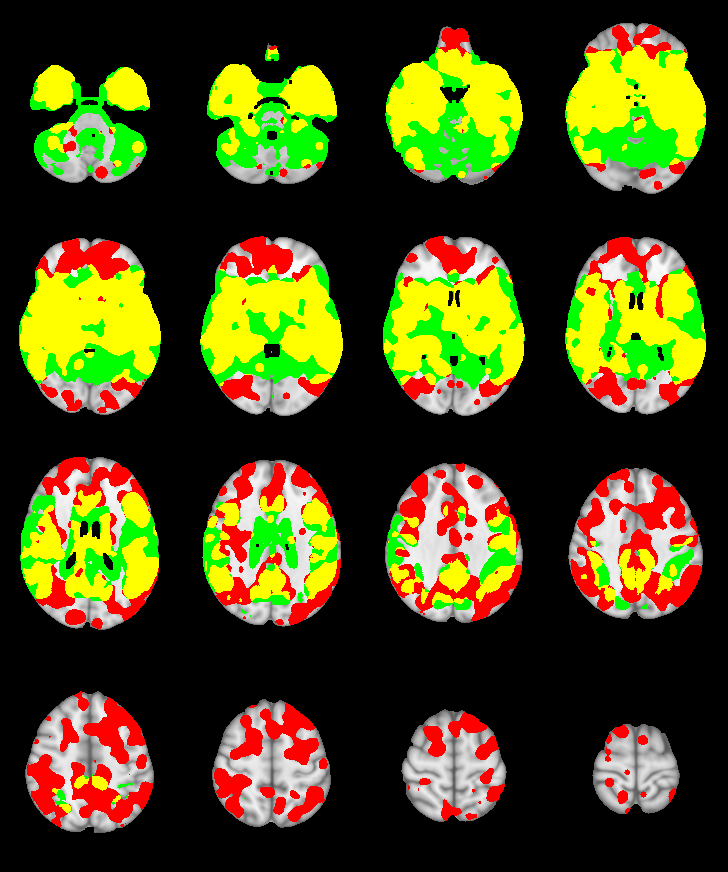
\includegraphics[
                    width=\slicewidth,
                    clip=true,
                    trim = 192mm 232mm 0mm 0mm
                ]{data/test_50.png}
            };
            \node[anchor=south, inner sep=\annotationpadding] at (axis cs: 0.7,0.5296) {
                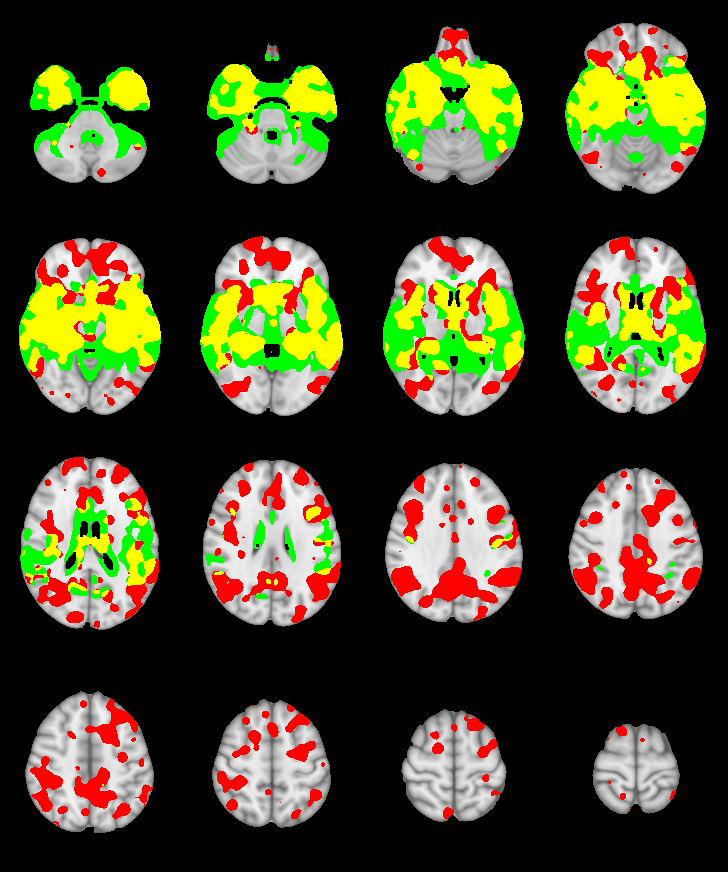
\includegraphics[
                    width=\slicewidth,
                    clip=true,
                    trim = 192mm 232mm 0mm 0mm
                ]{data/test_70.png}
            };
            \node[anchor=south, inner sep=\annotationpadding] at (axis cs: 0.9,0.4291) {
                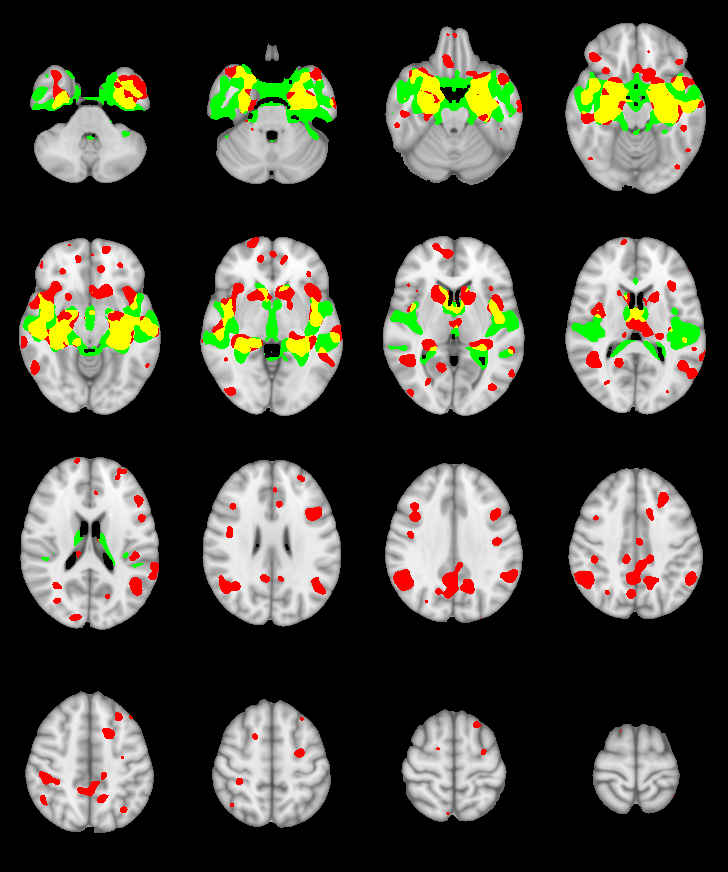
\includegraphics[
                    width=\slicewidth,
                    clip=true,
                    trim = 192mm 232mm 0mm 0mm
                ]{data/test_90.png}
            };
            % Legend
            \ifnum#1=1
                \node[
                    anchor=south west,
                    draw=black,
                    fill=white,
                    minimum width=3.45cm,
                    minimum height=1.22cm
                ] at (axis cs: 0.015, 0.015) {};
                \node[
                    circle,
                    draw=imagesdice,
                    fill=imagesdice,
                    anchor=south west,
                    inner sep=\legendnodesep
                ] (rwnode) at (axis cs: 0.035, 0.045) {};
                \node[anchor=west, text depth=0] (rw) at (rwnode.east) {\legendsize{Randomized images}};
                \node[
                    circle,
                    draw=weightsdice,
                    fill=weightsdice,
                    anchor=south,
                    inner sep=\legendnodesep
                ] (rinode) at ($ (rwnode.north) + (0, \legenddistance) $) {};
                \node[anchor=west, text depth=0] at (rinode.east) {\legendsize{Randomized weights}};
                \node[
                    circle,
                    draw=sexdice,
                    fill=sexdice,
                    anchor=south,
                    inner sep=\legendnodesep
                ] (sexnode) at ($ (rinode.north) + (0, \legenddistance) $) {};
                \node[anchor=west, text depth=0] at (sexnode.east) {\legendsize{Sex}};
                \node[
                    circle,
                    draw=dementiadice,
                    fill=dementiadice,
                    anchor=south,
                    inner sep=\legendnodesep
                ] (demnode) at ($ (sexnode.north) + (0, \legenddistance) $) {};
                \node[anchor=west, text depth=0] at (demnode.east) {\legendsize{Dementia}};
            \fi
        \end{axis}
    \end{tikzpicture}
}

\newsavebox{\dicebox}
\sbox{\dicebox}{
    \diceplot{0}
}
\newsavebox{\diceall}
\sbox{\diceall}{
    \diceplot{1}
}

\begin{frame}{Explainable dementia classification: Validation}
    \begin{tikzpicture}
        \node[] at (-5.25, 3.5) {};
        \node[] at (5.25, -3.5) {};

        \visible<1>{
			\node[
				minimum height=0.41\textwidth,
				minimum width=0.32\textwidth,
				fill=black,
                anchor=west
			] (box1) at (-5.25, 0) {};
			\node[anchor=south] at (box1.south) {
				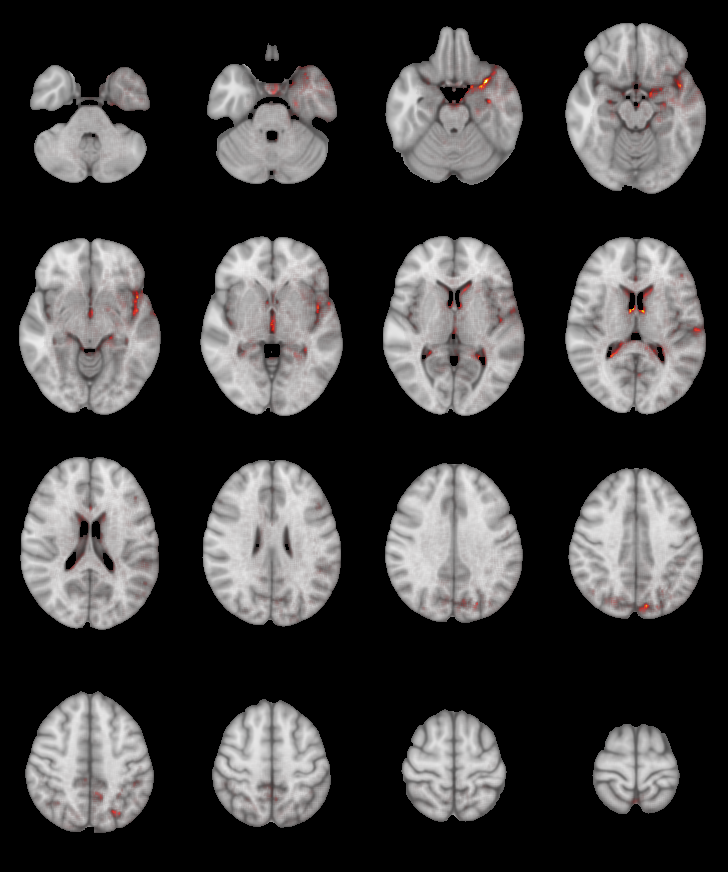
\includegraphics[width=0.31\textwidth]{data/subject1.png}
			};
			\node[anchor=north,inner sep=2pt, text=white, font=\footnotesize] at (box1.north) {Patient 1};

			\node
				[minimum height=0.41\textwidth,
				minimum width=0.32\textwidth,
				fill=black,
				anchor=west
			] (box2) at ($ (box1.east) + (0.05,0) $) {};
			\node[anchor=south] at (box2.south) {
				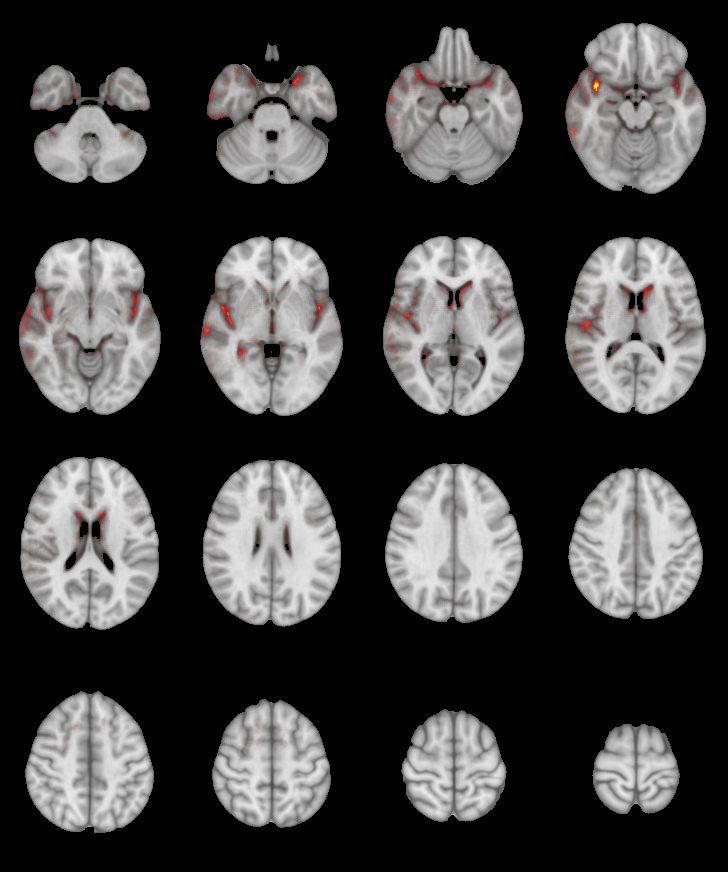
\includegraphics[width=0.31\textwidth]{data/subject2.png}
			};
			\node[anchor=north,inner sep=3pt, text=white, font=\footnotesize] at (box2.north) {Partient 2};

			\node
				[minimum height=0.41\textwidth,
				minimum width=0.32\textwidth,
				fill=black,
				anchor=west
			] (box3) at ($ (box2.east) + (0.05,0) $) {};
			\node[anchor=south] at (box3.south) {
				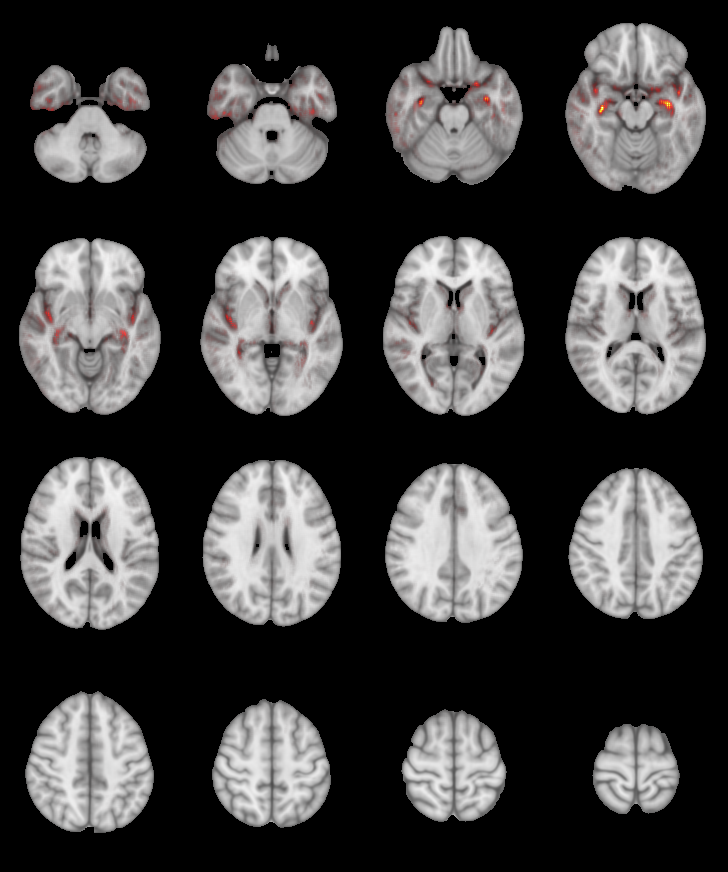
\includegraphics[width=0.31\textwidth]{data/subject3.png}
			};
			\node[anchor=north,inner sep=3pt, text=white, font=\footnotesize] at (box3.north) {Patient 3};
        }
        \visible<2-3>{
            \node[label={[text depth=0]above:LRP}] at (-2.25, 0) {
				
\includegraphics[width=0.31\textwidth]{data/dementia.png}
			};
        }
        \visible<3>{
			\node[label={[text depth=0]above:GingerALE}] at (2.25, 0) {
				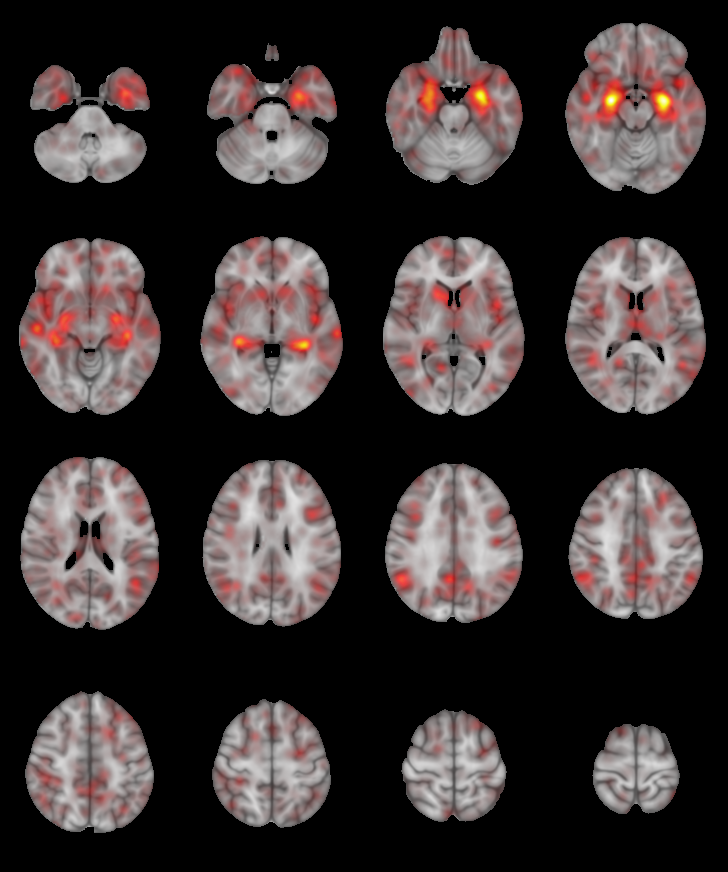
\includegraphics[width=0.31\textwidth]{data/ALE.png}
			};
        }
        \visible<4>{
            \node[
                minimum height=0.45\textwidth,
                minimum width=0.32\textwidth,
                fill=black,
                anchor=west
            ] (box1) at (-5.25, 0) {};
            \node[anchor=south] at ($ (box1.south) + (0, 0.3) $) {
                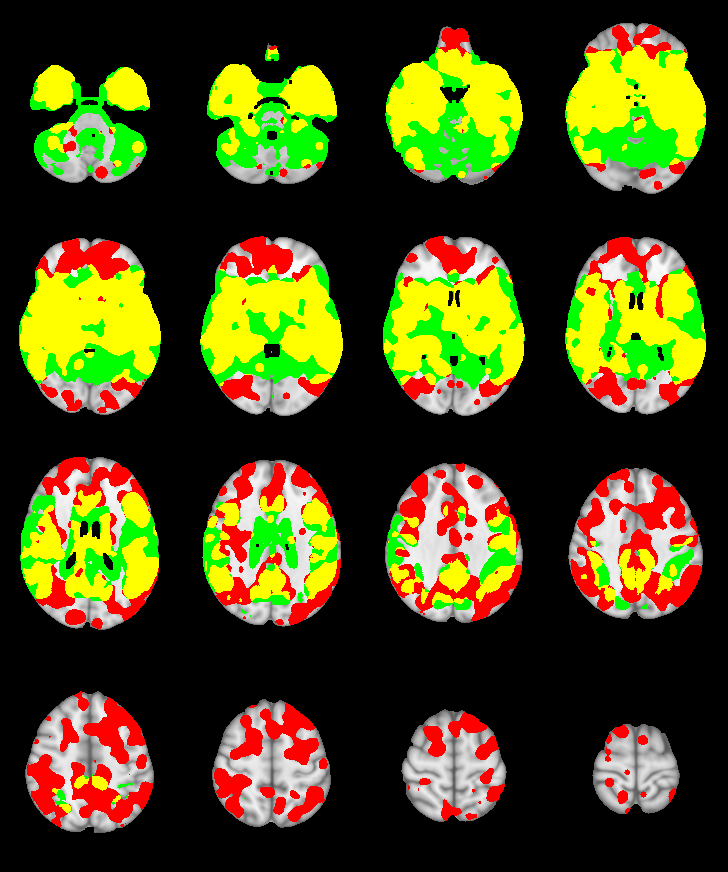
\includegraphics[width=0.31\textwidth]{data/test_50.png}
            };
            \node[anchor=north,inner sep=3pt, text=white, font=\footnotesize] at (box1.north) {50th percentile};

            \node
                [minimum height=0.45\textwidth,
                minimum width=0.32\textwidth,
                fill=black,
                anchor=west
            ] (box2) at ($ (box1.east) + (0.05,0) $) {};
            \node[anchor=south] at ($ (box2.south) + (0, 0.3) $) {
                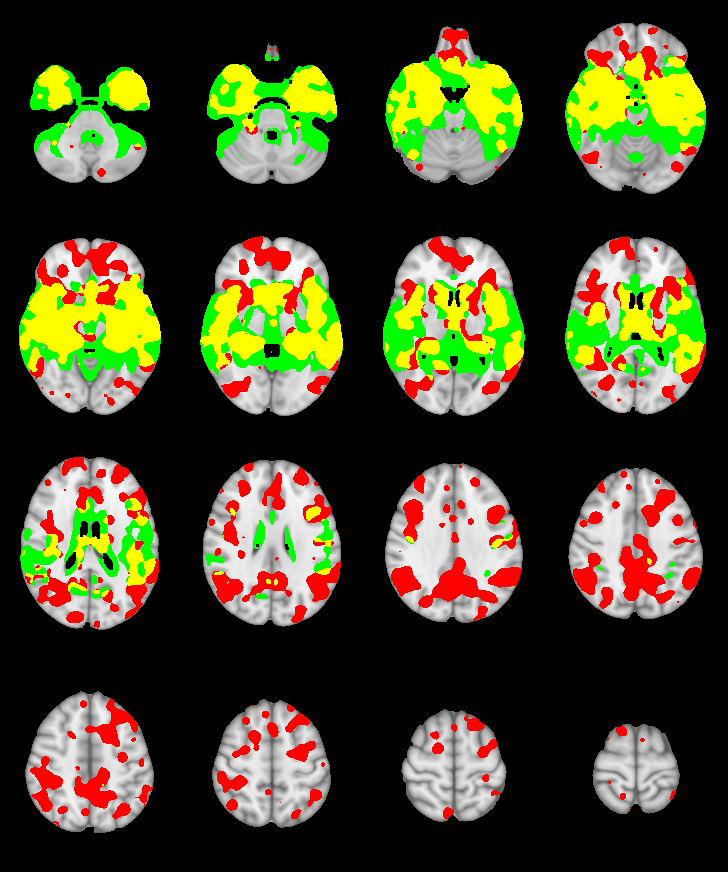
\includegraphics[width=0.31\textwidth]{data/test_70.png}
            };
            \node[anchor=north,inner sep=3pt, text=white, font=\footnotesize] at (box2.north) {70th percentile};

            \node
                [minimum height=0.45\textwidth,
                minimum width=0.32\textwidth,
                fill=black,
                anchor=west
            ] (box3) at ($ (box2.east) + (0.05,0) $) {};
            \node[anchor=south] at ($ (box3.south) + (0, 0.3) $) {
                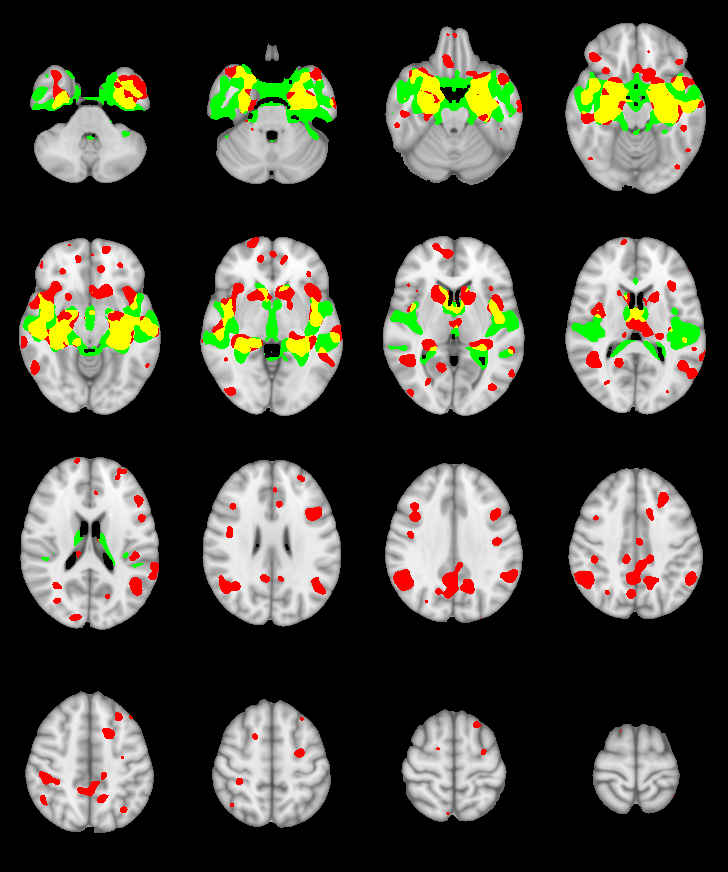
\includegraphics[width=0.31\textwidth]{data/test_90.png}
            };
            \node[anchor=north,inner sep=3pt, text=white, font=\footnotesize] at (box3.north) {90th percentile};

            \node[anchor=south, inner sep=0pt, text depth=0] (overlap) at ($ (box2.south) + (0.1, 0.15) $) {\textcolor{white}{\scriptsize{Overlap}}};
            \node[anchor=east, inner sep=2pt, fill=yellow] (overlap-box) at ($ (overlap.west) + (-0.07, 0) $) {};
            \node[anchor=east, inner sep=0pt,text depth=0] (lrp) at ($ (overlap-box.west) + (-0.2, 0) $) {\textcolor{white}{\scriptsize{LRP}}};
            \node[anchor=east, inner sep=2pt, fill=green] at ($ (lrp.west) + (-0.07, 0) $) {};
            \node[anchor=west, inner sep=2pt, fill=red] (ale-box) at ($ (overlap.east) + (0.2, 0) $) {};
            \node[anchor=west, inner sep=0pt, text depth=0] at ($ (ale-box.east) + (0.07, 0) $) {\textcolor{white}{\scriptsize{ALE}}};
        }
        \visible<5>{
            \node[] at (0, 0) {
                \usebox{\dicebox}
            };
        }
        \visible<6>{
            \node[] at (0, 0) {
                \usebox{\diceall}
            };
        }
    \end{tikzpicture}
\end{frame}

\newcommand{\prognostic}[1]{
    \begin{tikzpicture}
        \begin{axis}[
            height=2.9cm,
            width=4.08cm,
            xmajorticks=false,
            xmin=0.5,
            xmax=5.5,
            ymin=0,
            ymax=1,
            ylabel=\footnotesize{AUC},
            ymajorticks=false,
            ymajorgrids=true
        ]
            \addplot[mark=*, draw=black, mark options={fill=baseline}] coordinates {
                (1, 0.506)
                (2, 0.474)
                (3, 0.536)
                (4, 0.529)
                (5, 0.515)
            };
            \ifnum#1>0
                \addplot[mark=*, draw=black, mark options={fill=preds}] coordinates {
                    (1, 0.666)
                    (2, 0.742)
                    (3, 0.797)
                    (4, 0.844)
                    (5, 0.889)
                };
            \fi
            \ifnum#1>1
                \addplot[mark=*, draw=black, mark options={fill=maps}] coordinates {
                    (1, 0.743)
                    (2, 0.786)
                    (3, 0.808)
                    (4, 0.867)
                    (5, 0.903)
                };
            \fi
        \end{axis}
    \end{tikzpicture}
}

\newsavebox{\prognosticbaseline}
\sbox{\prognosticbaseline}{
    \prognostic{0}
}
\newsavebox{\prognosticpredictions}
\sbox{\prognosticpredictions}{
    \prognostic{1}
}
\newsavebox{\prognosticheatmaps}
\sbox{\prognosticheatmaps}{
    \prognostic{2}
}

\newcommand{\mciconcept}[1]{
    \begin{tikzpicture}
        \begin{axis}[
            height=0.6\textwidth,
            width=0.8\textwidth,
            xlabel={Age},
            ylabel={Cognitive function},
            ticks=none,
            axis x line=bottom,
            axis y line=left,
            y axis line style={-|},
            xmin=0,
            xmax=1.4,
            ymin=0,
            ymax=1,
            clip=false
        ]
            \addplot[draw=healthy-default, smooth, line width=4pt, opacity=0.5] coordinates {
                (0, 0.9)
                (0.25, 0.87)
                (0.5, 0.77)
                (0.6, 0.72)
                (0.8, 0.63)
                (0.9, 0.72)
                (1.4, 0.67)
            };
            \addplot[draw=controls-default, smooth, line width=4pt, opacity=0.5] coordinates {
                (0, 0.9)
                (0.25, 0.87)
                (0.5, 0.77)
                (0.6, 0.72)
                (0.8, 0.63)
                (0.9, 0.61)
                (1.4, 0.54)
            };
            \addplot[draw=cases-default, smooth, line width=4pt, opacity=0.5] coordinates {
                (0, 0.9)
                (0.25, 0.87)
                (0.5, 0.77)
                (0.6, 0.72)
                (0.8, 0.625)
                (1.1, 0.48)
                (1.4, 0.3)
            };
            \addplot[dashed] coordinates {
                (0, 0.65)
                (1.4, 0.65)
            };
            \addplot[dashed] coordinates {
                (0, 0.4)
                (1.4, 0.4)
            };
            \node[anchor=south west] at (axis cs: 0, 0.64) {\footnotesize{Normal cognition}};
            \node[anchor=north west] at (axis cs: 0, 0.66) {\footnotesize{Mild cognitive impairment}};
            \node[anchor=north west] at (axis cs: 0, 0.41) {\footnotesize{Dementia}};

            \ifnum#1=0
                \node[anchor=west] at (axis cs: 1.4, 0.67) {\textcolor{healthy-default}{\footnotesize{Improving (n=80)}}};
                \node[anchor=west] at (axis cs: 1.4, 0.53) {\textcolor{controls-default}{\footnotesize{Stable (n=754)}}};
                \node[anchor=west] at (axis cs: 1.4, 0.3) {\textcolor{cases-default}{\footnotesize{Progressive (n=354)}}};
            \fi
            \ifnum#1>1
                \draw[-stealth, red, thick] (axis cs: 0.8, 0.8) -- (axis cs: 0.8, 0.67);
                \node[anchor=south] at (axis cs: 0.8, 0.8) {\textcolor{red}{\footnotesize{t}}};
            \fi

            \ifnum#1>2
                \draw[densely dotted] (axis cs: 0.9, 0.8) -- (axis cs: 0.9, 0.3);
                \draw[densely dotted] (axis cs: 1, 0.8) -- (axis cs: 1, 0.3);
                \draw[densely dotted] (axis cs: 1.1, 0.8) -- (axis cs: 1.1, 0.3);
                \draw[densely dotted] (axis cs: 1.2, 0.8) -- (axis cs: 1.2, 0.3);
                \draw[densely dotted] (axis cs: 1.3, 0.8) -- (axis cs: 1.3, 0.3);
                \node[anchor=south] at (axis cs: 0.9, 0.8) {\footnotesize{t+1}};
                \node[anchor=south] at (axis cs: 1, 0.8) {\footnotesize{t+2}};
                \node[anchor=south] at (axis cs: 1.1, 0.8) {\footnotesize{t+3}};
                \node[anchor=south] at (axis cs: 1.2, 0.8) {\footnotesize{t+4}};
                \node[anchor=south] at (axis cs: 1.3, 0.8) {\footnotesize{t+5}};
            \fi

            \ifnum#1=4
                \node[] at (axis cs: 1.05, 0.155) {
                    \usebox{\prognosticbaseline}
                };
                \node[anchor=west] at (axis cs: 1.34, 0.158) {\footnotesize{0.51}};
            \fi
            \ifnum#1=5
                \node[] at (axis cs: 1.05, 0.155) {
                    \usebox{\prognosticpredictions}
                };
			    \node[anchor=west] at (axis cs: 1.34, 0.261) {\footnotesize{0.88}};
            \fi
            \ifnum#1=6
                \node[] at (axis cs: 1.05, 0.155) {
                    \usebox{\prognosticheatmaps}
                };
			    \node[anchor=west] at (axis cs: 1.34, 0.262) {\footnotesize{0.90}};
            \fi

        \end{axis}
    \end{tikzpicture}
}

\newsavebox{\mcitrajectories}
\sbox{\mcitrajectories}{
    \mciconcept{0}
}
\newsavebox{\mcioutline}
\sbox{\mcioutline}{
    \mciconcept{1}
}
\newsavebox{\mcitimepoint}
\sbox{\mcitimepoint}{
    \mciconcept{2}
}
\newsavebox{\mcifuture}
\sbox{\mcifuture}{
    \mciconcept{3}
}
\newsavebox{\mcibaseline}
\sbox{\mcibaseline}{
    \mciconcept{4}
}
\newsavebox{\mcipredictions}
\sbox{\mcipredictions}{
    \mciconcept{5}
}
\newsavebox{\mciheatmaps}
\sbox{\mciheatmaps}{
    \mciconcept{6}
}

\newsavebox{\mcigroups}
\sbox{\mcigroups}{
    \begin{tikzpicture}
        \begin{axis}[
            height=0.6\textwidth,
            width=1.1\textwidth,
            xmin=0,
            xmax=1,
            ymin=0,
            ymax=1.05,
            ymajorticks=false,
            xtick pos=bottom,
            xlabel={Predicted probability of dementia},
        ]
            \addplot[draw=none, name path=zero] coordinates {(0, 0) (1, 0)};
            \addplot[
                draw=healthy-default,
                very thick,
                name path=improved
            ] table [
                col sep=comma,
                x=points,
                y=improved,
            ] {data/distributions.csv};

            \addplot[healthy-default, opacity=0.2] fill between [
                of=zero and improved
            ];

            \addplot[
                draw=controls-default,
                very thick,
                name path=stable
            ] table [
                col sep=comma,
                x=points,
                y=stable
            ] {data/distributions.csv};

            \addplot[controls-default, opacity=0.2] fill between [
                of=zero and stable
            ];

            \addplot[
                draw=cases-default,
                very thick,
                name path=declined
            ] table [
                col sep=comma,
                x=points,
                y=declined
            ] {data/distributions.csv};

            \addplot[cases-default, opacity=0.2] fill between [
                of=zero and declined
            ];

            \addplot[
                only marks,
                fill=healthy-default,
                mark options={mark size=3pt},
                draw=healthy-default
            ] coordinates {(0.105, 4.418/7.838)};

            \addplot[
                only marks,
                fill=controls-default,
                mark options={mark size=3pt},
                draw=controls-default
            ] coordinates {(0.333, 0.592/7.838)};

            \addplot[
                only marks,
                fill=cases-default,
                mark options={mark size=3pt},
                draw=cases-default
            ] coordinates {(0.649, 0.829/7.838)};

            \node[anchor=south] at (axis cs: 0.649, 0.95/7.838) {\scriptsize{\textcolor{cases-default}{0.649}}};
            \node[anchor=south] at (axis cs: 0.333, 0.72/7.838) {\scriptsize{\textcolor{controls-default}{0.333}}};
            \node[anchor=west] at (axis cs: 0.11, 4.418/7.838) {\scriptsize{\textcolor{healthy-default}{0.105}}};

            \node[circle, inner sep=2pt, label={[text depth=0]right:Improving}, fill=healthy-default!20, draw=healthy-default] (imci) at (axis cs: 0.76, 0.98) {};
            \node[circle, inner sep=2pt, anchor=north, label={[text depth=0]right:Stable}, fill=controls-default!20, draw=controls-default] (smci) at ($ (imci.south) + (0, -3.5) $) {};
            \node[circle, inner sep=2pt, anchor=north, label={[text depth=0]right:Progressive}, fill=cases-default!20, draw=cases-default] (pmci) at ($ (smci.south) + (0, -3.5) $) {};
        \end{axis}
    \end{tikzpicture}
}

\newsavebox{\mcimixed}
\sbox{\mcimixed}{
    \newcommand{\linestyle}{densely dotted}
    \newcommand{\diffx}{-5}
    \newcommand{\legendy}{0.92}

    \begin{tikzpicture}
        \begin{axis}[
            height=7cm,
            width=9cm,
            xmin=-9,
            xmax=0,
            ymin=0,
            ymax=1,
            xtick={-8, -6, -4, -2, 0},
            xticklabels={8, 6, 4, 2, 0},
            xlabel=Years before diagnosis,
            ylabel=Group-wise mean\\dementia prediction,
            error bars/y dir=both,
            error bars/y explicit,
            xmajorgrids=true,
            xtick style={draw=none},
            ytick pos=left,
            ylabel style={align=center, font=\normalfont\linespread{0.9}\selectfont},
            grid style={draw=gray!20},
            xlabel style={text depth=0pt}
        ]
            \addplot[
                cases-default,
                scatter,
                scatter/use mapped color={
                    draw=cases-default,
                    fill=cases-default
                },
                visualization depends on=\thisrow{declining_size}\as\size,
                scatter/@pre marker code/.append style={
                    /tikz/mark size=\size ^ 0.3,
                    /tikz/mark color=cases-default
                }
            ] table [
                col sep=comma,
                x=year,
                y=declining_mean,
            ] {data/yearly_trajectories.csv};
            \addplot[
                controls-default,
                scatter,
                scatter/use mapped color={
                    draw=controls-default,
                    fill=controls-default
                },
                visualization depends on=\thisrow{declining_size}\as\size,
                scatter/@pre marker code/.append style={
                    /tikz/mark size=\size ^ 0.3,
                    /tikz/mark color=cases-default
                }
            ] table [
                col sep=comma,
                x=year,
                y=stable_mean,
            ] {data/yearly_trajectories.csv};
            \node[circle, minimum size=5.4pt, fill=gray, inner sep=0pt, anchor=north west] (n25mark) at (axis cs: -8.5, 0.94) {};
            \coordinate (label) at (axis cs: -11.37, 0.87);
            \addplot[
                cases-default,
                scatter,
                scatter/use mapped color={
                    draw=cases-default,
                    fill=cases-default
                },
                mark size=2.5pt
            ] coordinates {
                (-3.6, 0.14)
            };
            \node[anchor=west, text depth=0] at (axis cs: -3.5, 0.14) {\small{Progressive}};
            \addplot[
                controls-default,
                scatter,
                scatter/use mapped color={
                    draw=controls-default,
                    fill=controls-default
                },
                mark size=2.5pt
            ] coordinates {
                (-3.6, 0.07)
            };
            \node[anchor=west, text depth=0] at (axis cs: -3.5, 0.07) {\small{Non-progressive}};
        \end{axis}
        \node[anchor=west, inner sep=0pt] (n25label) at ($ (n25mark.east) + (0.05, 0) $) {\small{n=25}};
        \node[anchor=west, circle, minimum size=8.5pt, fill=gray, inner sep=0pt] (n100mark) at ($ (n25label.east) + (0.1, 0) $) {};
        \node[anchor=west, inner sep=0pt] (n100label) at ($ (n100mark.east) + (0.05, 0) $) {\small{100}};
        \node[anchor=west, circle, minimum size=12pt, fill=gray, inner sep=0pt] (n250mark) at ($ (n100label.east) + (0.1, 0) $) {};
        \node[anchor=west, inner sep=0pt] (n250label) at ($ (n250mark.east) + (0.05, 0) $) {\small{250}};
    \end{tikzpicture}
}

\newcommand{\mriwidth}{2.2cm}
\newcommand{\gap}{0.00cm}

\newcommand{\survivalplot}[4]{
    \begin{tikzpicture}
        \def\ylabel{Healthy\\fraction}
        \def\xlabel{Age}
        \def\ytick{{0, 0.2, 0.4, 0.6, 0.8, 1.0}}

        \ifnum#4=0
            \def\ylabel{}
            \def\xlabel{}
            \def\ytick{}
        \fi

        \begin{axis}[
            height=3cm,
            width=1.71 * \mriwidth,
            ylabel style={
                align=center,
                font=\tiny\linespread{0.8}\selectfont,
                at={(axis description cs:-0.2,0.5)}
            },
            xlabel style={
                font=\tiny\selectfont,
                at={(axis description cs: 0.5, -0.0)}
            },
            ylabel=\ylabel,
            xlabel=\xlabel,
            every tick label/.append style={font=\tiny},
            xtick pos=bottom,
            ymin=0,
            ymax=1,
            xmin=62,
            xmax=95,
            ytick=\ytick,
            ytick style={draw=none},
            xtick style={draw=none},
            ymajorgrids=true,
            xmajorticks=false,
            grid style={line width=.5pt, draw=gray!25},
        ]

        \addplot[controls-default, very thick] table [col sep=comma, x=age, y=baseline] {#1};
        \addplot[healthy-default, very thick] table [col sep=comma, x=age, y=fifth] {#1};
        \addplot[cases-default, very thick] table [col sep=comma, x=age, y=ninetyfifth] {#1};
        \node[anchor=south west,font=\tiny] at (axis cs: 62, 0.2) {
            $\beta\mathrm{=}#2$
        };
        \node[anchor=south west,font=\tiny] at (axis cs: 62, 0.0) {
            $p\mathrm{=}#3$
        };
        \end{axis}
    \end{tikzpicture}
}

\newsavebox{\firstsurvival}
\sbox{\firstsurvival}{
    \survivalplot{data/survival/survival_0.csv}{0.68}{1.59\times10^{-66}}{1}
}
\newsavebox{\secondsurvival}
\sbox{\secondsurvival}{
    \survivalplot{data/survival/survival_2.csv}{-0.24}{4.40\times10^{-26}}{0}
}
\newsavebox{\thirdsurvival}
\sbox{\thirdsurvival}{
    \survivalplot{data/survival/survival_3.csv}{0.22}{2.31\times10^{-20}}{0}
}

\newcommand{\survivalanalysis}[1]{
    \hspace{-1.3cm}
    \begin{tikzpicture}
        \node[] at (-2.3, 2.1) {};
        \node[] at (8.8, -3.6) {};

        \node[label={[text depth=0pt]above:Component 0}] (first) at (0, 0) {
            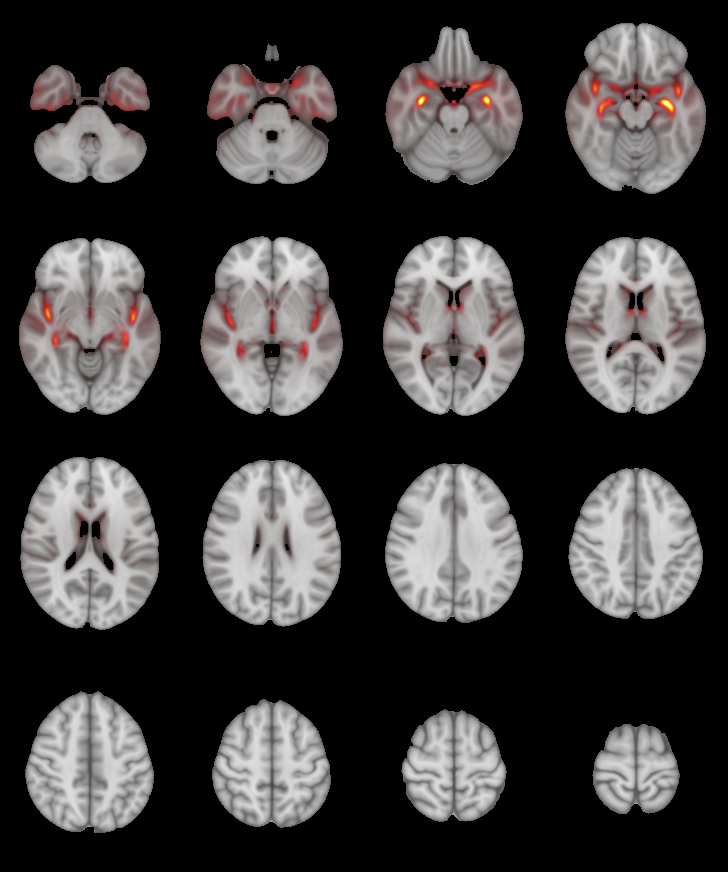
\includegraphics[
                width=\mriwidth,
                clip=true,
                trim = 192mm 232mm 0mm 0mm
            ]{data/components/component_0.png}
        };

        \node[anchor=west, label={[text depth=0pt]above:Component 1}] (second) at ($ (first.east) + (\gap, 0) $) {
            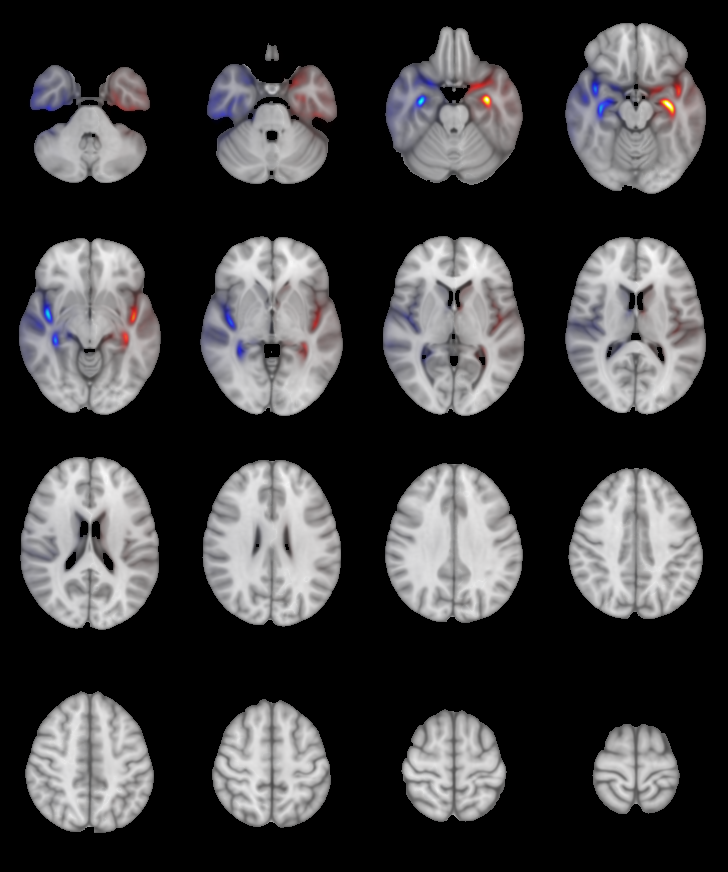
\includegraphics[
                width=\mriwidth,
                clip=true,
                trim = 192mm 232mm 0mm 0mm
            ]{data/components/component_1.png}
        };

        \node[anchor=west, label={[text depth=0pt]above:Component 2}] (third) at ($ (second.east) + (\gap, 0) $) {
            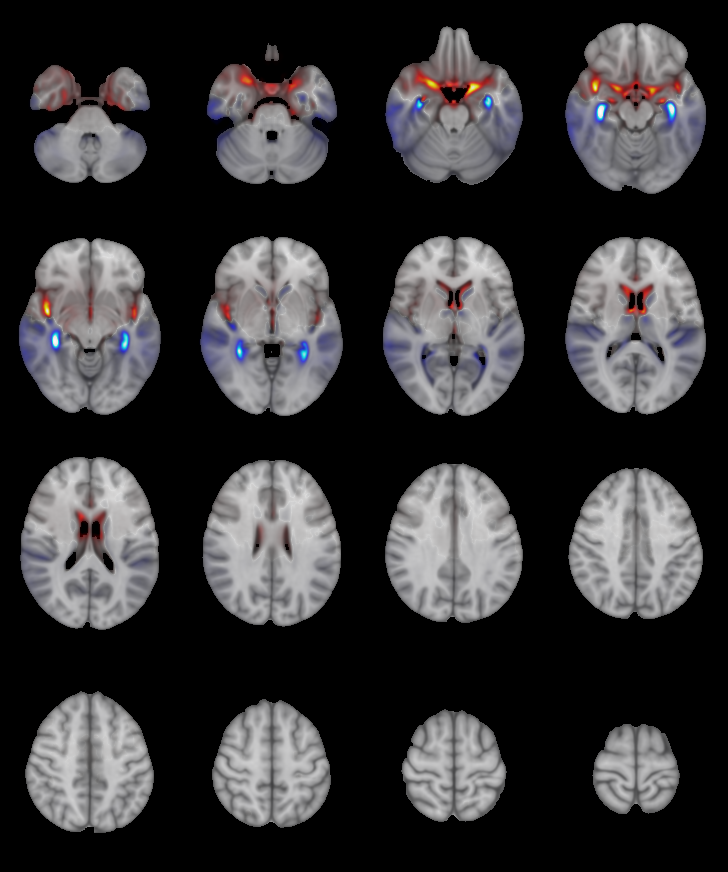
\includegraphics[
                width=\mriwidth,
                clip=true,
                trim = 192mm 232mm 0mm 0mm
            ]{data/components/component_2.png}
        };

        \node[anchor=west, label={[text depth=0pt]above:Component 3}] (fourth) at ($ (third.east) + (\gap, 0) $) {
            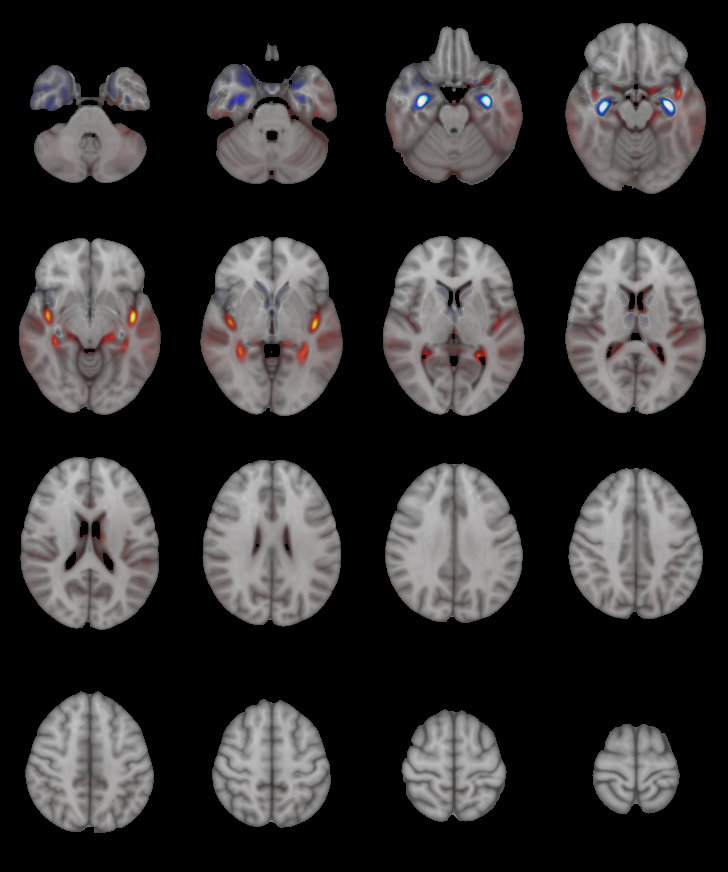
\includegraphics[
                width=\mriwidth,
                clip=true,
                trim = 192mm 232mm 0mm 0mm
            ]{data/components/component_3.png}
        };

        \ifnum#1>0
            \node[anchor=north west] (first-survival) at ($ (first.south west) + (-1.3, 0.35) $) {
                \usebox{\firstsurvival}
            };
            \node[anchor=north west] (third-survival) at ($ (third.south west) + (-0.91, 0.158) $) {
                \usebox{\secondsurvival}
            };
            \node[anchor=north west] (fourth-survival) at ($ (fourth.south west) + (-0.91, 0.158) $) {
                \usebox{\thirdsurvival}
            };
            \node[anchor=north, inner sep=2pt] (legend-header) at ($ (second.south) - (0, 0) $) {\scriptsize{\underline{Percentiles}}};
            \node[anchor=north west, inner sep=1pt] (tenth) at ($ (legend-header.south east) - (0.83, 0) $) {\scriptsize{5th}};
            \node[anchor=north west, inner sep=1pt] (fiftieth) at (tenth.south west) {\scriptsize{50th}};
            \node[anchor=north west, inner sep=1pt] (ninetyeth) at (fiftieth.south west) {\scriptsize{95th}};
            \draw[draw=healthy-default, very thick, text depth=0] ($ (tenth.west) + (-0.43, 0) $) -- ($ (tenth.west) + (-0.05, 0) $);
            \draw[draw=controls-default, very thick, text depth=0] ($ (fiftieth.west) + (-0.43, 0) $) -- ($ (fiftieth.west) + (-0.05, 0) $);
            \draw[draw=cases-default, very thick, text depth=0] ($ (ninetyeth.west) + (-0.43, 0) $) -- ($ (ninetyeth.west) + (-0.05, 0) $);
        \fi
    \end{tikzpicture}
}

\newsavebox{\survivalpca}
\sbox{\survivalpca}{
    \survivalanalysis{0}
}
\newsavebox{\survivalcurves}
\sbox{\survivalcurves}{
    \survivalanalysis{1}
}

\newcommand{\correlationplot}[4]{
    \begin{tikzpicture}
        \begin{axis}[
            height=1.71 * \mriwidth,
            width=1.71 * \mriwidth,
            xmajorticks=false,
            ylabel=#3,
            ytick={0, 2, 4, 6, 8},
            yticklabels=#2,
            xmin=-1,
            xmax=17,
            ymin=0,
            ymax=9,
            every tick label/.append style={font=\tiny},
            ytick pos=left,
            scatter/classes={
                ADNI_EF={color0, draw=black},
                ADNI_MEM={color1, draw=black},
                CDCARE={color2, draw=black},
                CDCOMMUN={color3, draw=black},
                CDGLOBAL={color4, draw=black},
                CDHOME={color5, draw=black},
                CDJUDGE={color6, draw=black},
                CDMEMORY={color7, draw=black},
                CDORIENT={color8, draw=black},
                FAQTOTAL={color9, draw=black},
                GDTOTAL={color10, draw=black},
                MMSCORE={color11, draw=black},
                NPISCORE={color12, draw=black},
                PHC_EXF={color13, draw=black},
                PHC_LAN={color14, draw=black},
                PHC_MEM={color15, draw=black},
                PHC_VSP={color16, draw=black}
            },
            y label style={at={(-0.1,0.5)}},
            ymajorgrids=true,
            ytick style={draw=none},
            clip=false,
            grid style={draw=gray!20},
            axis line style={draw=gray!70}
        ]
            \addplot[
                only marks,
                scatter,
                scatter src=explicit symbolic
            ] table [
                col sep=comma,
                x=index,
                y=component_#1,
                meta=symptom
            ] {data/correlations.csv};
            \addplot[dashed,red, thick] coordinates {
                (-1, 2.76)
                (17, 2.76)
            };
            #4
        \end{axis}
    \end{tikzpicture}
}

\newsavebox{\firstcorrelations}
\sbox{\firstcorrelations}{%
    \correlationplot{0}{{0, 2, 4, 6, 8}}{\scriptsize{$-log_{10}(p)$}}{
        \node[] at (axis cs: 14, 6.19) {\tiny{PHC\_LAN}};
    }
}
\newsavebox{\secondcorrelations}
\sbox{\secondcorrelations}{%
    \correlationplot{1}{{,,}}{{}}{
        \node[] at (axis cs: 9, 3.74) {\tiny{FAQTOTAL}};
    }
}
\newsavebox{\thirdcorrelations}
\sbox{\thirdcorrelations}{%
    \correlationplot{2}{{,,}}{{}}{
        \node[] at (axis cs: 0, 6.44) {\tiny{ADNI\_EF}};
        \node[] at (axis cs: 13, 7.95) {\tiny{PHC\_EXF}};
    }
}
\newsavebox{\fourthcorrelations}
\sbox{\fourthcorrelations}{%
    \correlationplot{3}{{,,}}{{}}{
        \node[] at (axis cs: 0, 9.02) {\tiny{ADNI\_EF}};
        \node[] at (axis cs: 13, 8.75) {\tiny{PHC\_EXF}};
        \node[] at (axis cs: 14, 5.84) {\tiny{PHC\_LAN}};
        \node[] at (axis cs: 6, 5.18) {\tiny{CDJUDGE}};
        \node[] at (axis cs: 11, 3.99) {\tiny{MMSCORE}};
    }
}

\newsavebox{\cognitivecorrelations}
\sbox{\cognitivecorrelations}{
    \begin{tikzpicture}
        \node[] (first) at (0, 0) {
            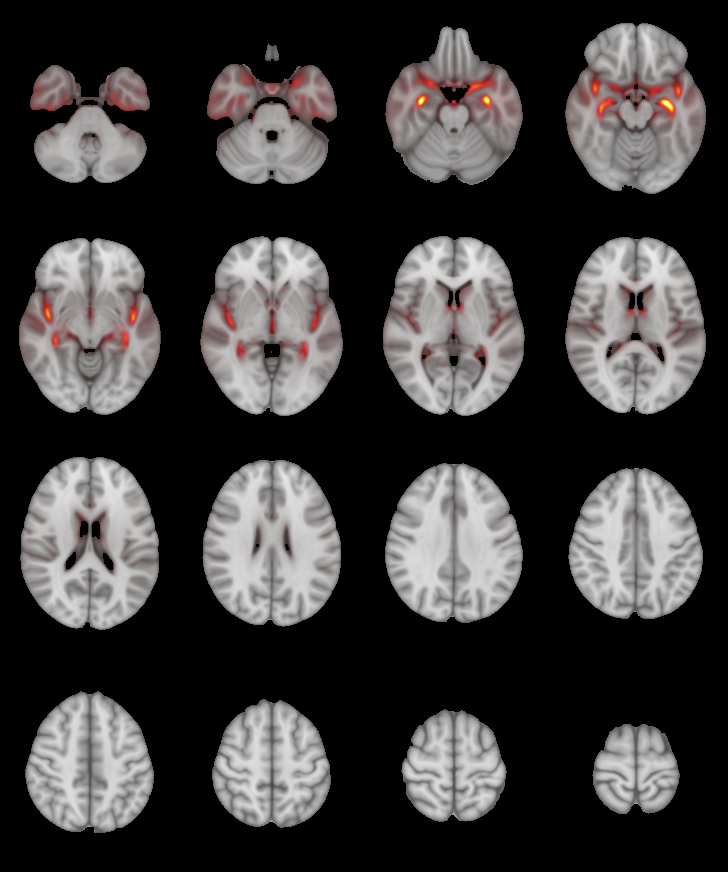
\includegraphics[
                width=\mriwidth,
                clip=true,
                trim = 192mm 232mm 0mm 0mm
            ]{data/components/component_0.png}
        };
        \node[anchor=north west] (first-correlation) at ($ (first.south west) + (-0.86, 0.1) $) {
            \usebox{\firstcorrelations}
        };

        \node[anchor=west] (second) at ($ (first.east) + (\gap, 0) $) {
            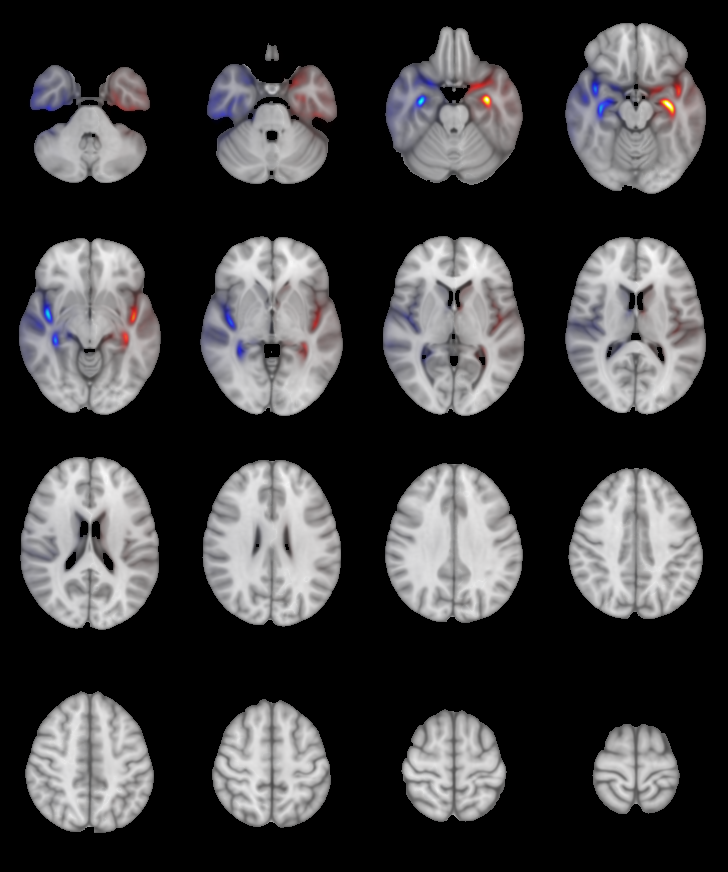
\includegraphics[
                width=\mriwidth,
                clip=true,
                trim = 192mm 232mm 0mm 0mm
            ]{data/components/component_1.png}
        };
        \node[anchor=north west] (second-correlation) at ($ (first-correlation.north east) - (0.76, 0) $) {
            \usebox{\secondcorrelations}
        };

        \node[anchor=west] (third) at ($ (second.east) + (\gap, 0) $) {
            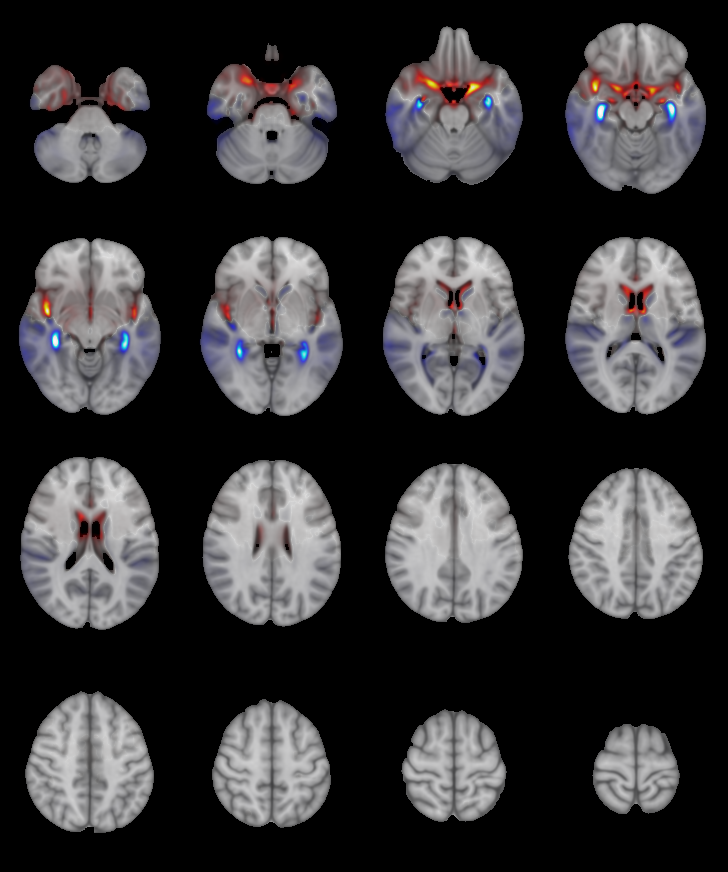
\includegraphics[
                width=\mriwidth,
                clip=true,
                trim = 192mm 232mm 0mm 0mm
            ]{data/components/component_2.png}
        };
        \node[anchor=north west] (third-correlation) at ($ (second-correlation.north east) - (0.71, 0) $) {
            \usebox{\thirdcorrelations}
        };

        \node[anchor=west] (fourth) at ($ (third.east) + (\gap, 0) $) {
            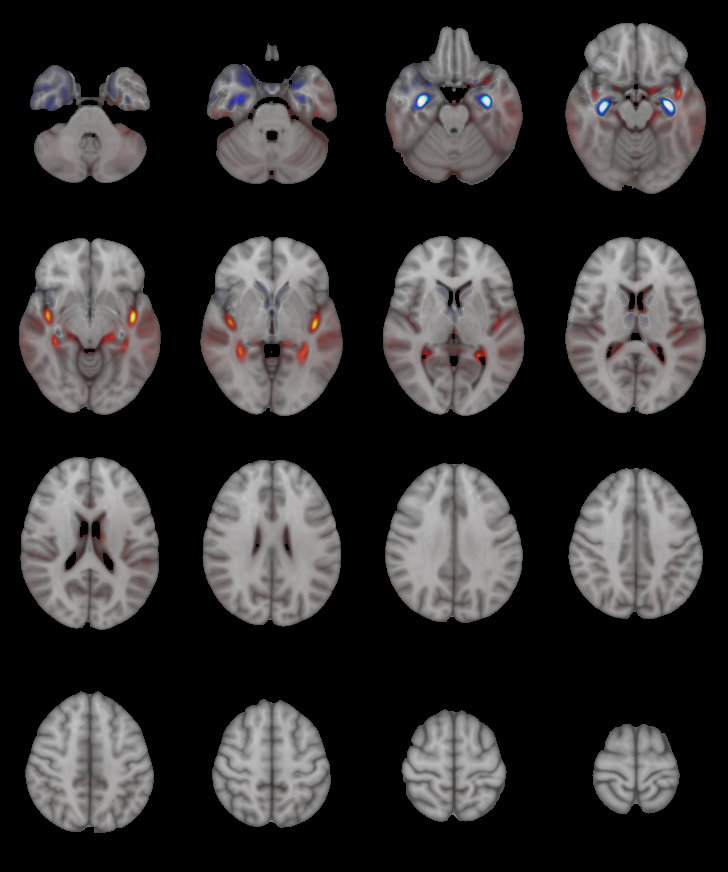
\includegraphics[
                width=\mriwidth,
                clip=true,
                trim = 192mm 232mm 0mm 0mm
            ]{data/components/component_3.png}
        };
        \node[anchor=north west] (fourth-correlation) at ($ (third-correlation.north east) - (0.74, -0.21) $) {
            \usebox{\fourthcorrelations}
        };
    \end{tikzpicture}
}

\begin{frame}{Explainable dementia classification: Application}
    \begin{tikzpicture}
        \node[draw=black] at (-5.25, 3.5) {};
        \node[draw=black] at (5.25, -3.5) {};

        \visible<1>{
            \node[] at (0, 0) {
                \usebox{\mcitrajectories}
            };
        }

        \visible<2>{
            \node[] at (0, 0) {
                \usebox{\mcigroups}
            };
        }
        \visible<3>{
            \node[] at (0, 0) {
                \usebox{\mcimixed}
            };
        }
        \visible<4>{
            \node[] at (0, 0) {
                \usebox{\survivalpca}
            };
        }
        \visible<5>{
            \node[] at (0, 0) {
                \usebox{\survivalcurves}
            };
        }
        \visible<6>{
            \node[] at (0, 0) {
                \usebox{\mcioutline}
            };
        }
        \visible<7>{
            \node[] at (0, 0) {
                \usebox{\mcitimepoint}
            };
        }
        \visible<8>{
            \node[] at (0, 0) {
                \usebox{\mcifuture}
            };
        }
        \visible<9>{
            \node[] at (0, 0) {
                \usebox{\mcibaseline}
            };
        }
        \visible<10>{
            \node[] at (0, 0) {
                \usebox{\mcipredictions}
            };
        }
        \visible<11>{
            \node[] at (0, 0) {
                \usebox{\mciheatmaps}
            };
        }
        \visible<12>{
            \node[] at (0, 0) {
                \usebox{\cognitivecorrelations}
            };
        }
        \visible<13>{
            \node[] at (0, 0) {
                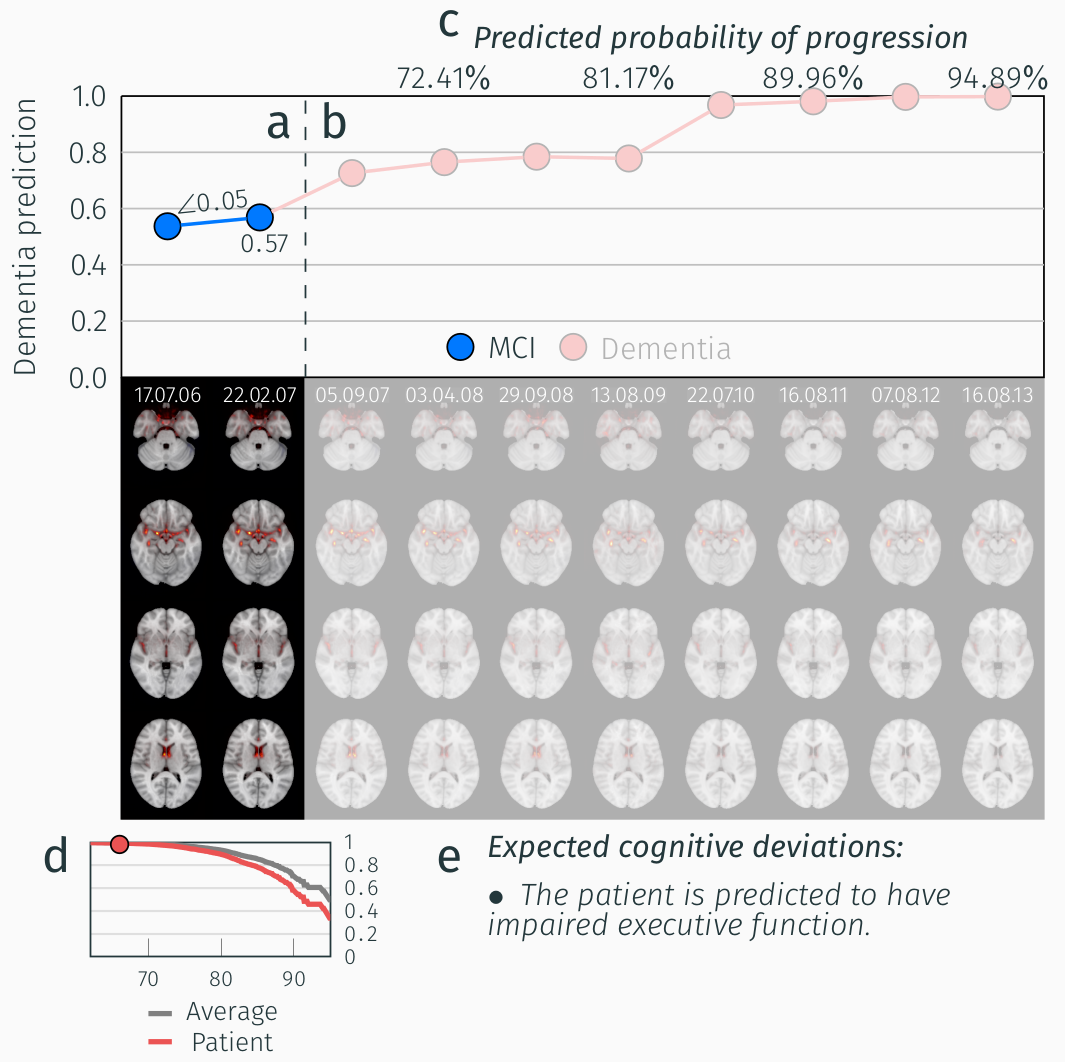
\includegraphics[height=7cm]{data/morphological.png}
            };
        }

    \end{tikzpicture}
\end{frame}
